


\tikzset{every picture/.style={line width=0.75pt}} %set default line width to 0.75pt

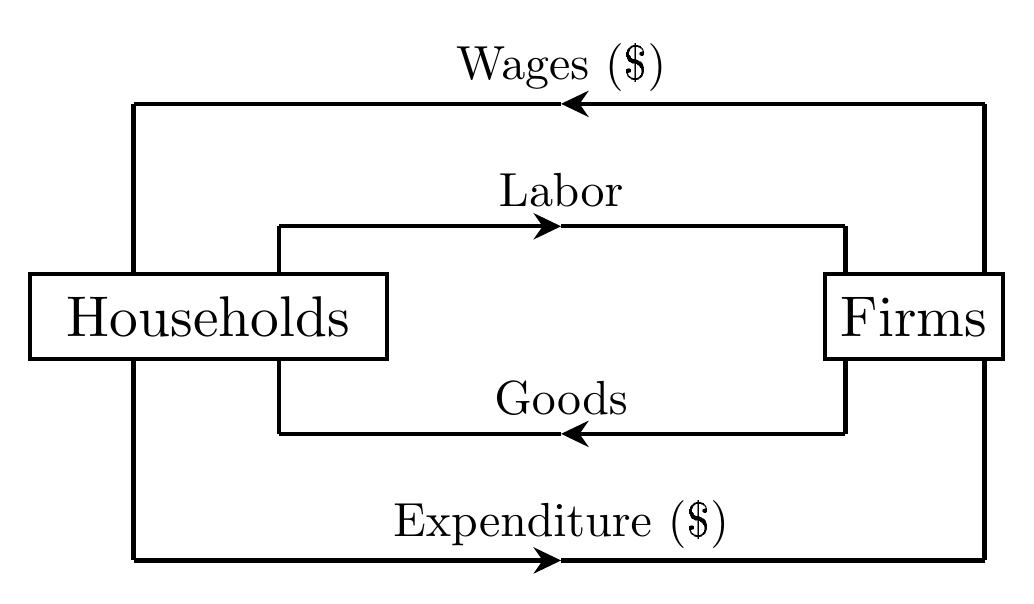
\begin{tikzpicture}[x=0.75pt,y=0.75pt,yscale=-1,xscale=1]
%uncomment if require: \path (0,300); %set diagram left start at 0, and has height of 300

%Straight Lines [id:da3142809335416301]
\draw [line width=1.5]    (124,59.5) -- (124,141) ;


%Straight Lines [id:da9626190695079444]
\draw [line width=1.5]    (124,182) -- (124,279.5) ;


%Straight Lines [id:da3345837970311947]
\draw [line width=1.5]    (124,279.5) -- (327,279.5) ;
\draw [shift={(330,279.5)}, rotate = 180] [fill={rgb, 255:red, 0; green, 0; blue, 0 }  ][line width=1.5]  [draw opacity=0] (13.4,-6.43) -- (0,0) -- (13.4,6.44) -- (8.9,0) -- cycle    ;

%Straight Lines [id:da01953277539539222]
\draw [line width=1.5]    (330,279.5) -- (534,279.5) ;


%Straight Lines [id:da7687846182646736]
\draw [line width=1.5]    (124,59.5) -- (330,59.5) ;


%Straight Lines [id:da44029552198348365]
\draw [line width=1.5]    (333,59.5) -- (534,59.5) ;

\draw [shift={(330,59.5)}, rotate = 0] [fill={rgb, 255:red, 0; green, 0; blue, 0 }  ][line width=1.5]  [draw opacity=0] (13.4,-6.43) -- (0,0) -- (13.4,6.44) -- (8.9,0) -- cycle    ;
%Straight Lines [id:da3663913301698425]
\draw [line width=1.5]    (534,59.5) -- (534,141) ;


%Straight Lines [id:da5032753193398922]
\draw [line width=1.5]    (534,182) -- (534,279.5) ;


%Straight Lines [id:da9932947895966895]
\draw [line width=1.5]    (194,182) -- (194,218.5) ;


%Straight Lines [id:da18539319752174643]
\draw [line width=1.5]    (194,118.5) -- (194,141) ;


%Straight Lines [id:da49775346522692754]
\draw [line width=1.5]    (194,118.5) -- (327,118.5) ;
\draw [shift={(330,118.5)}, rotate = 180] [fill={rgb, 255:red, 0; green, 0; blue, 0 }  ][line width=1.5]  [draw opacity=0] (13.4,-6.43) -- (0,0) -- (13.4,6.44) -- (8.9,0) -- cycle    ;

%Straight Lines [id:da34816473919309443]
\draw [line width=1.5]    (330,118.5) -- (467,118.5) ;


%Straight Lines [id:da1253109371352814]
\draw [line width=1.5]    (467,118.5) -- (467,141) ;


%Straight Lines [id:da5483581319301252]
\draw [line width=1.5]    (467,182) -- (467,218.5) ;


%Straight Lines [id:da11360523157716229]
\draw [line width=1.5]    (194,218.5) -- (330,218.5) ;


%Straight Lines [id:da04502522469810577]
\draw [line width=1.5]    (333,218.5) -- (467,218.5) ;

\draw [shift={(330,218.5)}, rotate = 0] [fill={rgb, 255:red, 0; green, 0; blue, 0 }  ][line width=1.5]  [draw opacity=0] (13.4,-6.43) -- (0,0) -- (13.4,6.44) -- (8.9,0) -- cycle    ;

% Text Node
\draw  [line width=1.5]   (74,141.5) -- (246,141.5) -- (246,182.5) -- (74,182.5) -- cycle  ;
\draw (160,162) node [scale=2.074] [align=left] {Households};
% Text Node
\draw  [line width=1.5]   (457,141.5) -- (543,141.5) -- (543,182.5) -- (457,182.5) -- cycle  ;
\draw (500,162) node [scale=2.074] [align=left] {Firms};
% Text Node
\draw (330,42) node [scale=1.7280000000000002] [align=left] {Wages (\$)};
% Text Node
\draw (330,101) node [scale=1.7280000000000002] [align=left] {Labor};
% Text Node
\draw (330,201) node [scale=1.7280000000000002] [align=left] {Goods};
% Text Node
\draw (330,262) node [scale=1.7280000000000002] [align=left] {Expenditure (\$)};


\end{tikzpicture}

